\documentclass[a4paper]{article}
\title{PhD Thesis}
\author{Fintan S. Nagle}



%BEGIN MATRIX GUMF
% Load TikZ
\usepackage{tikz}
\usetikzlibrary{matrix,decorations.pathreplacing,calc}

% Set various styles for the matrices and braces. It might pay off to fiddle around with the values a little bit
\pgfkeys{tikz/mymatrixenv/.style={decoration=brace,every left delimiter/.style={xshift=3pt},every right delimiter/.style={xshift=-3pt}}}
\pgfkeys{tikz/mymatrix/.style={matrix of math nodes,left delimiter=[,right delimiter={]},inner sep=2pt,column sep=1em,row sep=0.5em,nodes={inner sep=0pt}}}
\pgfkeys{tikz/mymatrixbrace/.style={decorate,thick}}
\newcommand\mymatrixbraceoffseth{0.5em}
\newcommand\mymatrixbraceoffsetv{0.2em}

% Now the commands to produce the braces. (I'll explain below how to use them.)
\newcommand*\mymatrixbraceright[4][m]{
    \draw[mymatrixbrace] ($(#1.north west)!(#1-#3-1.south west)!(#1.south west)-(\mymatrixbraceoffseth,0)$)
        -- node[left=2pt] {#4} 
        ($(#1.north west)!(#1-#2-1.north west)!(#1.south west)-(\mymatrixbraceoffseth,0)$);
}
\newcommand*\mymatrixbraceleft[4][m]{
    \draw[mymatrixbrace] ($(#1.north east)!(#1-#2-1.north east)!(#1.south east)+(\mymatrixbraceoffseth,0)$)
        -- node[right=2pt] {#4} 
        ($(#1.north east)!(#1-#3-1.south east)!(#1.south east)+(\mymatrixbraceoffseth,0)$);
}
\newcommand*\mymatrixbracetop[4][m]{
    \draw[mymatrixbrace] ($(#1.north west)!(#1-1-#2.north west)!(#1.north east)+(0,\mymatrixbraceoffsetv)$)
        -- node[above=2pt] {#4} 
        ($(#1.north west)!(#1-1-#3.north east)!(#1.north east)+(0,\mymatrixbraceoffsetv)$);
}
\newcommand*\mymatrixbracebottom[4][m]{
    \draw[mymatrixbrace] ($(#1.south west)!(#1-1-#3.south east)!(#1.south east)-(0,\mymatrixbraceoffsetv)$)
        -- node[below=2pt] {#4} 
        ($(#1.south west)!(#1-1-#2.south west)!(#1.south east)-(0,\mymatrixbraceoffsetv)$);
}

%END MATRIX GUMF
 
 
 

\usepackage[mediumspace,mediumqspace,Grey,squaren]{SIunits}
\usepackage{subfigure}
 \usepackage{graphicx}
 \usepackage{mathtools}
 \usepackage{amsmath}
 \usepackage{setspace}
 \usepackage{tikz}

\newenvironment{enoomerate}{
\begin{enumerate}
  \setlength{\itemsep}{1pt}
  \setlength{\parskip}{0pt}
  \setlength{\parsep}{0pt}}{\end{enumerate}
}

\newenvironment{itemise}{
\begin{itemize}
  \setlength{\itemsep}{1pt}
  \setlength{\parskip}{0pt}
  \setlength{\parsep}{0pt}}{\end{itemize}
}



\newcommand{\up}[1]{\ensuremath{^{\textrm{#1}}}}
\newcommand{\down}[1]{\ensuremath{_{\textrm{#1}}}}

\newcommand{\Xangstrom}{\r{a}ngstr\"{o}m}


\newcommand{\Xth}{\up{\tiny{th}}}
\newcommand{\st}{\up{\small{st}}}
\newcommand{\nd}{\up{\small{nd}}}
\newcommand{\rd}{\up{\small{rd}}}

\newcommand{\Xeta}{\textit{et al }}
\newcommand{\Xiv}{\textit{in vivo }}
\newcommand{\Xxv}{\textit{ex vivo }}
\newcommand{\Xis}{\textit{in silico }}

\newcommand{\etal}{\textit{et al }}
\newcommand{\invivo}{\textit{in vivo }}
\newcommand{\exvivo}{\textit{ex vivo }}
\newcommand{\insilico}{\textit{in silico }}
\newcommand{\invitro}{\textit{in vitro }}

\newcommand{\um}{\micro m}

\newcommand{\xa}{\textit{a) }}
\newcommand{\xb}{\textit{b) }}
\newcommand{\xc}{\textit{c) }}
\newcommand{\xd}{\textit{d) }}
\newcommand{\xe}{\textit{e) }}

%DOCUMENT-SPECIFIC COMMANDS

 \newcommand{\pcatwo}{PCA\up{2} }




%\begin{figure}[htp]
%\centering
%\includegraphics[scale=0.5]{img/bubbles.png}
%\caption{Bubbles in the right atrium (RA) and vena cava (VC) of a guinea pig after decompression from 0.4MPa. From \cite{daniels1980detection}. Approximate scale: the area shown   in the image measures several mm across.}
%\label{bubbles}
%\end{figure}

%width = /textwidth

\begin{document}
\maketitle

\begin{center}
Supervisors: Alan Johnston and Peter McOwan
\\
$n$ words as counted by  the TeXcount script at \texttt{http://app.uio.no/ifi/texcount/index.html}.
\vspace{3cm}

%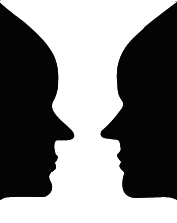
\includegraphics[scale=0.5]{img/twofaces.png}

\vspace{3cm}

\textit{Acknowledgements}\\
...
\end{center}


\pagebreak


\tableofcontents



\pagebreak

\section{Literature review}

\section{Terms}

\section{The overall goal}


\section{Modularity}

The property of modularity is the possibility to divide a system into multiple components!

\section{Forms of neural coding}

\begin{itemise}
\item \textbf{Single neuron activation}. The firing of a single neuron can convey binary information.
\item \textbf{Single spike frequency} can code a real-valued quantity.
\item \textbf{Spike frequency across multiple neurons} can code relative information between two real-valued quantities.
\item \textbf{Connection patterns} between neurons (the existence of a connection, or its strength) can code complex information, but this information cannot be extracted without activating the neurons and monitoring the outputs.
\end{itemise}

\section{Static and dynamic faces are processed differently}

The first evidence of a difference in the perception of expression between static and dynamic faces was found in 1991\cite{humphreys1993expression}.


\section{Identity vs. expression}

There is a substantial body of evidence that identity (information which is invariant within individuals) and expression (information which is invariant across perceived emotional states) are processed differently. On the high level, identity judgement and expression judgement have been observed to be doubly dissociated in prosopagnosics\cite{archer1994movement}. However, this observation may not allow us to generalise deductions to the normally-functional population, as prosopagnosics may have developed alternative recognition strategies such as non-holistic feature recognition (as is used to recognise classes of objects for which we do not possess a specialised representation or processing system).

On a slightly lower level, judgement reaction times differ depending on whether expression or identity is being judged; when judging identity, familiar faces are matched faster, but familiarity confers no advantage when judging expression\cite{bruce1986understanding}. This could imply that the computation of identity is intrinsically more complex or that other neural actions such as memory retrieval of biographical data are triggered.

On the lowest level, it is possible to find individual neurons which are receptive to either identity or expression\cite{hasselmo1989role}. Multidimensional scaling methods on their spike train data allow stimuli to be classified in either identity or expression space solely by neural response.

However, the location in one test subject of a small number of individual neurons which correlate with a particular condition provides no information about the algorithmics of face processing; it simply demonstrates that the brain can judge identity and expression at some level (which is intuitively obvious) and that this information can be coded by neural activation as opposed to connection patterning or higher-level codes such as spike train phase.

\section{Correlates between the two decouplings}

It is tempting to connect the identity-expression dichotomy with the static-dynamic dichotomy, as dynamic faces have constant identity but changing expression. This would be erroneous, as static faces can vary in both expression and identity.

\section{Object perception}

\section{Visual perception as dimensionality reduction}

Visual perception creates percepts from visual input. Photons arrive on the retina and induce signals in the optic nerve, which then pass to the LGN, dorsal and ventral visual pathways, and eventually effect conscious perception (such as when we perceive a face) or motor control (such as when we press a button to indicate that we have seen a face).

The number of photons arriving per unit time is so high that they cannot all be losslessly recorded, as shown by the reduced information capacity of the optic nerve\cite{wolff1993computing} compared to the retina, so information is compressed before dispatch. Motion representations are a simple form of compression; rather than recording the positions of a dot at each time-step (1,2,3,...,99,100), we can simply record its initial position (1) and speed (1 unit per second). Averaging is another simple compressor, as is nonlinear activation of cone cells (which require several afferent photons to change their membrane potential).


The bandwidth of the optic nerve is also smaller than that of incoming light signals, and this is dealt with by retinal adaptation.

%Insert from adaptation book here

These forms of compression can all be seen as transfer functions from low- to higher-level representations. The ultimate low-level representation of visual input is to record every photon arriving on the retina, but as this is impractical, optic nerve representations are compressed.

The process continues as we move further away from the retina and into the early visual system. Colour perception is another compression strategy, allowing any combination of wavelengths to be described by three coordinates in colour spaces like RGB, HSV or LAB.

Compression is evident in Marr's theory of vision, as in \cite{marr1978representation}:

"A representation is a formal system for making explicit certain entities or types of information, together with a specification of how the system does this. And I shall call the result of using a representation to describe a given entity a description of the entity in that representation."

Provided that Marr's "result" contains less information than his "entities or types of information," representation is precisely a process of compression.

Different types of representation record and miss different types of information. For example, neurons in V5 are sensitive to motion but not to colour; neurons in FFA are sensitive to faces but not houses. Many early visual centres are retinotopically mapped, keeping account of the position on the retina of a stimulus. This information, however, is not always useful: maintaining a map requires separate channels for each part of the visual field, even those which are not of interest.

In a retinotopically-mapped representation, it is easy to compare objects in the same position by simply subtracting or Pearson-correlating the corresponding areas. However, if the same object is present in the top-left of map A and the bottom-right of map B, comparing the two maps will not detect object identity.

In reality, object recognition is position-invariant: we are able to track an object as it moves around on the retina, and also to compare objects in different positions in the map. How position-invariant representations are built is a key problem in understanding the brain\cite{stringer2000position}.

Position-invariance is an important quality of object percepts, but is it sufficient to say that something is perceived as an object? Object perception is often associated with two other properties: spatiotemporal extent, and a canonical coordinate frame.

\paragraph{Spatiotemporal extent}
Most objects have spatial extent: defined borders. Prominent work on segmentation\cite{kiper1996cortical,grossberg1987role,atkinson1992visual,riseman1977computational,li1999visual} and figure-ground separation\cite{kelly2000neural,grossberg1993figure,grossberg19943} (which is simply segmentation from the background) underlines how important this process is to vision. Segmentation is task-specific: although we \textit{can} segment this object:
\begin{center}
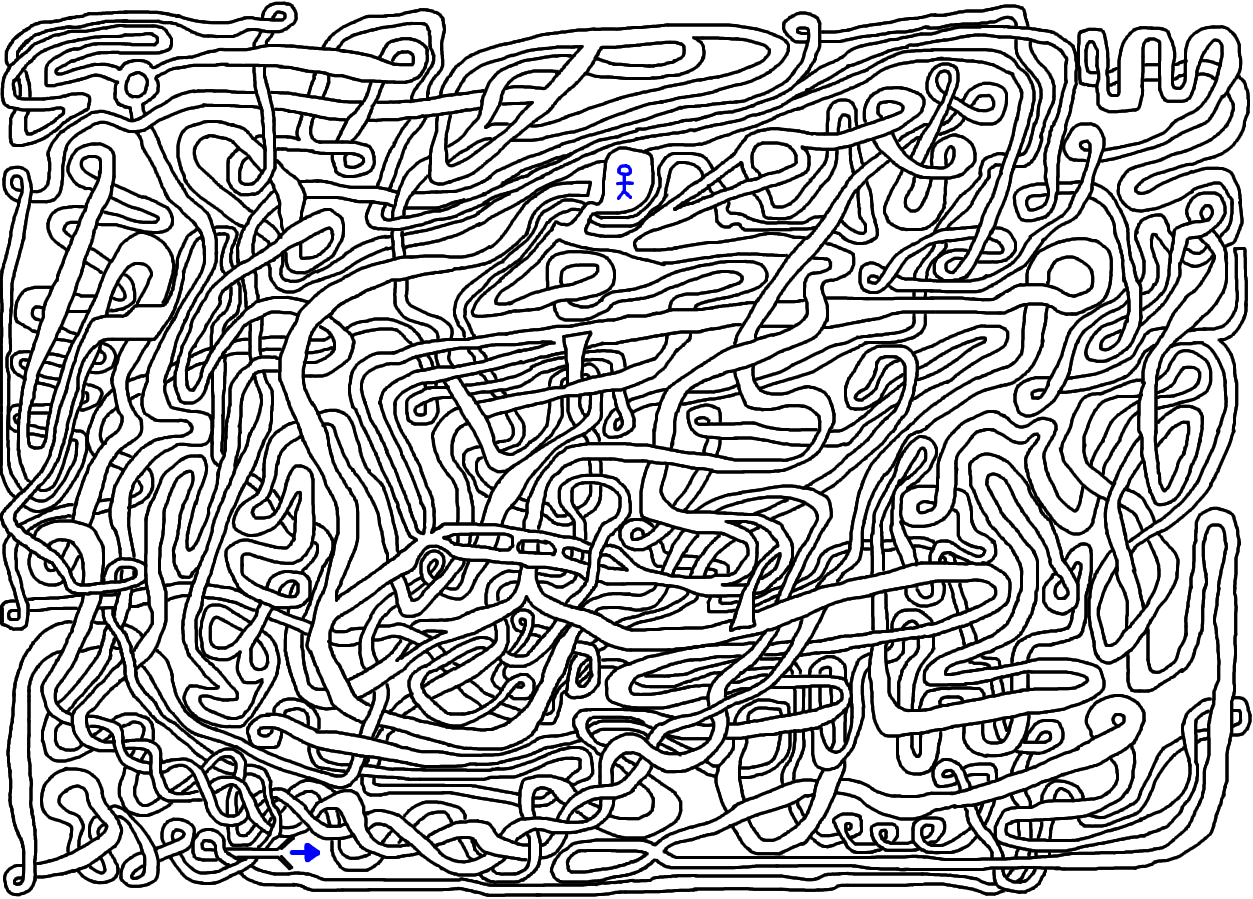
\includegraphics[width=0.3\textwidth]{img/maze.png}
\end{center}

we do not automatically perform that complex computation (and cannot without scanning the fovea over the image, as it is too detailed) unless engaged in a task which requires it, like copying the object.

When reasoning about dynamic stimuli, some objects have temporal extent: they appear at a certain moment, then disappear. Temporal extent is often task-sensitive. For example, a changing traffic light can be seen either as three permanent ``light" objects which change colour, or as ``red-light", ``yellow-light" and ``green-light" objects which appear when they illuminate and disappear when they darken.

\paragraph{Canonical coordinate frames}

Translation is not the only transformation under which objects are invariant: they also preserve their identity under 2D or 3D rotation and scaling. Marr pointed out that many objects are more easily recognised from certain points of view and inferred that they possess principal axes\cite{marr1982vision}. This property allows different objects of the same class to be compared; their principal axes can be aligned, allowing features to be registered.

In summary, objects are percepts which admit position invariance and have defined extent. However, all visual input is not segmented into objects. One of the main stimulus classes which we do not segment consists of textures.

\subsection{Textures}

There is much work on texture perception\cite{}, individuation\cite{} and classification\cite{}

Textures differ from objects 

\section{Representations}

It is important to note that there is never a unique representation of a visual stimulus, and it makes no sense to speak of "the" representation of a face or a house. Representations of a scene include:

Retinal photon trace (similar to a digital camera image)
Optic nerve representation
Neural recordings from V1
Neural recordings from the FFA
A verbal description of a scene
A written description of the scene

In terms of size, representations range from the very small (a recording from a single face-sensitive neuron can be taken to represent the presence or absence of a face in its receptive field) to the very large (such as Gallant's reconstruction of visual input from multivoxel MR imaging\cite{naselaris2009bayesian}).

The Marrean view sees representations as processes. Like other processes, such as functions, they can be composed so that information flows through them sequentially. Visual information flows from the retina to a single face-sensitive neuron as follows:

Retina - optic nerve - visual centres - FFA - neuron of interest

\subsection{Levels}

Representations can be seen to operate on different levels. We say that we move "up" from a low-level representation (the retina, or image space) to a high-level representation (FFA neurons, or face space). "Top-down control" indicates that cognitive representations accessible to consciousness are influencing low-level representations like motor neuron activity.

This up-and-down metaphor is very imprecise, despite being very common in the literature (over 369,000 results for the search "top-down control vision" on the Google Scholar literature search engine). It can generally be interpreted in two ways.

\paragraph{1. Top-bottom as distance from consciousness}
This view sees representations as being organised according to their interaction with consciousness. Qualia, intentions and percepts are the most high-level representations, as they are consciously accessible. Early visual system representations are seen as lower-level as they can be hidden from consciousness by processes like masking, crowding and adaptation. We refer to this as the \textbf{awareness scale}.

\paragraph{2. Top-bottom as representational information}
This view sees representations as being organised according to their information content, or entropy. Consider our two alternative codes for the 1D positions of a moving point, R1:(1,2 3,4,...,99,100) and R2:(start=1, speed=1). Although they describe the same thing, R1 contains 50 times more information than R2 (100 numbers compared to 50). We refer to this as the \textbf{information scale}.

These two metaphors describe completely different things, yet are mixed under the monikers "top-down" and "bottom-up." It is necessary to be very clear about which one we mean.

\subsection{Operations on representations}

Matching. Two representations can be compared for identity. This usually happens on two representations of equal information level








%the pca spacetime

%the thing needs to include more expressions! possibly let's use the emotional.

%the idea that we may have to process things in terms of the neural movements- we are very good at copying expressions, could this mean something? the input and output systems are likely to be linked, no?

\begin{singlespace}
\begin{footnotesize}
\begin{twocolumn}
\bibliographystyle{unsrt}
\bibliography{references,bib_litreview}
\end{twocolumn}
\end{footnotesize}
\end{singlespace}
\newpage

Appendices here

\end{document}



